\chapter{Multivariate Normal Model}

Now we have seen a little bit about how Bayesian models work when the sampling random variable maps to a 1-dimensional real number. In this chapter, through the perspective of multivariate normal, we take a tour around the world when 
\begin{equation*}
    X: \mathcal{F} \rightarrow \mathbb{R}^p
\end{equation*}

\section{Semi-Conjugate Prior}
Semi-conjugate modeling requires parameters to be independent to each other, which is easier to begin with. In high dimension cases, each data point/sample looks like this
\begin{equation*}
    Y_i = (Y_{i1}, \ldots, Y_{ip})^T \in \mathbb{R}^p
\end{equation*}

As a semi-conjugate case, the following plot illustrates how will we structure this model. While both $\vec{\theta}, \Sigma$ depends on some latent variables, but they are not implicitely connected in any way. Firstly, we will talk about how we are going to model the prior of $\vec{\theta}$ and leave $\Sigma$'s latent for now. 

\begin{center}
    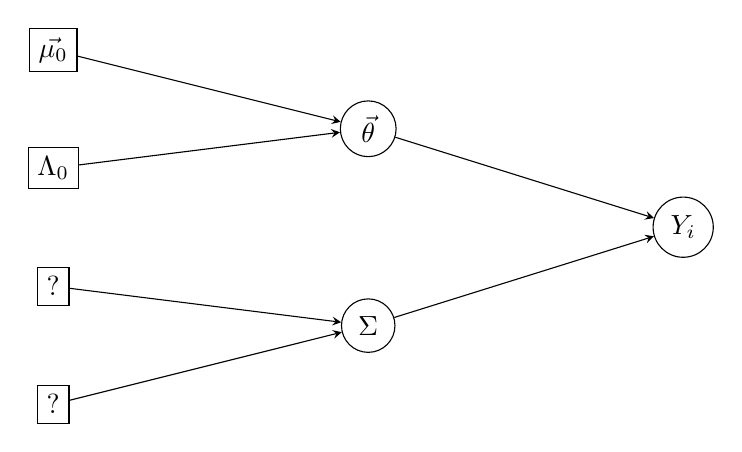
\begin{tikzpicture}[>=stealth, node distance=2cm and 4cm]
    
        % Define nodes in the first column (left)
        \node[draw, rectangle] (A1) at (0,0) {$\vec{\mu_0}$};
        \node[draw, rectangle] (A2) at (0,-1.5) {$\Lambda_0$};
        \node[draw, rectangle] (A3) at (0,-3) { ? };
        \node[draw, rectangle] (A4) at (0,-4.5) { ? };
        
        % Define nodes in the second column (middle)
        \node[draw, circle] (B1) at (4,-1) {$\vec{\theta}$};
        \node[draw, circle] (B2) at (4,-3.5) {$\Sigma$};
        
        % Define node in the third column (right)
        \node[draw, circle] (C1) at (8,-2.25) {$Y_{i}$};
        
        % Draw arrows connecting the first column to the second column
        \draw[->] (A1) -- (B1);
        \draw[->] (A2) -- (B1);
        \draw[->] (A3) -- (B2);
        \draw[->] (A4) -- (B2);
        
        % Draw arrows connecting the second column to the third column
        \draw[->] (B1) -- (C1);
        \draw[->] (B2) -- (C1);
    
    \end{tikzpicture}
\end{center}

\subsection{$\theta$ as Multivariate Normal}
In the 1-dimension case, we modeled $\theta$ as a normal. As a high-dimensional generalization, we choose to model $\vec{\theta}$ as multivariate normal:
\begin{equation*}
    \vec{\theta} \sim MVN(\mu_0, \Lambda_0)
\end{equation*}
If we dive deeper into its pdf, we have the following:
\begin{align*}
    p(\vec{\theta}) &= (2\pi)^{-p/2}|\Lambda_0|^{-1/2} \exp \big( -\frac{1}{2}(\theta - \mu_0)^T \Lambda_0^{-1}(\theta - \mu_0) \big) \\
    &\propto \exp \big( -\frac{1}{2}\theta^T\Lambda_0^{-1}\theta + \frac{1}{2}\theta^T\Lambda_0^{-1}\mu_0 + \frac{1}{2}\mu_0^T\Lambda_0^{-1}\theta - \frac{1}{2}\mu_0^T\Lambda_0^{-1}\mu_0 \big) \\
    &\propto \exp \big( -\frac{1}{2}\theta^T\Lambda_0^{-1}\theta + \theta^T\Lambda_0^{-1}\mu_0 \big) \\ 
    &= \exp \big( -\frac{1}{2}\theta^TA_0\theta + \theta^T b_0 \big)
\end{align*}
where we reparametized $A_0 = \Lambda_0^{-1}$ and $b_0 = A_0\mu_0 = \Lambda_0^{-1}\mu_0$.

As a direct consequence of the reparametrization, we have 
\begin{equation*}
    \vec{\theta} \sim MVN(A_0^{-1}b_0, A_0^{-1})
\end{equation*}

\subsection*{Joint Sampling Model}
Now, assuming we have known $\Sigma$, then our sampling model can be written as 
\begin{align*}
    p(\vec{\theta} | \vec{Y}, \theta, \Sigma) &= \Pi_{i=1}^n (2\pi)^{-p/2} |\Sigma|^{-\frac{1}{2}} \exp \big( -\frac{1}{2}(Y_i - \vec{\theta})^T \Sigma^{-1}(Y_i - \vec{\theta}) \big) \\
    &\propto \exp \big( -\frac{n}{2}\theta^T\Sigma^{-1}\theta + \theta^T\Sigma^{-1}\sum_{i=1}^n Y_i - \frac{1}{2}\sum_{i=1}^n(Y_i^T\Sigma^{-1}Y_i) \big) \\
    &\propto \exp \big( -\frac{1}{2}\theta^TA_1\theta + \theta^Tb_1 \big)
\end{align*}
where we reparametized $A_1 = n\Sigma^{-1}$ and $b_1 = \Sigma^{-1}\sum_{i=1}^nY_i = n\Sigma^{-1}\bar{Y}$

\subsection*{Posterior}
With the sampling and prior, we now formulate the posterior:
\begin{align*}
    p(\vec{\theta} | \vec{Y}, \Sigma) &\propto p(\vec{Y} | \theta, \Sigma) \cdot p(\theta) \\
    &\propto \exp \big( -\frac{1}{2}\theta^TA_1\theta + \theta^Tb_1 \big) \cdot \exp \big( -\frac{1}{2}\theta^TA_0\theta + \theta^Tb_0 \big) \\
    &= \exp \big( -\frac{1}{2}\theta^T(A_0 + A_1)\theta + \theta^T(b_0 + b_1) \big)
\end{align*}
Notice the first line where we used Bayes' rule, we have $p(\theta | \Sigma) = p(\theta)$ because we are modeling the semi-conjugate case. In conclusion, we have obtained the posterior as
\begin{equation*}
    \vec{\theta} | \vec{Y}, \Sigma \sim MVN(A_n^{-1}b_n, A_n^{-1})
\end{equation*}
where $A_n = A_0 + A_1 = \Lambda_0^{-1} + n\Sigma^{-1}$ and $b_n = b_0 + b_1 = \Lambda_0^{-1}\mu_0 + n\Sigma^{-1}\bar{Y}$

\subsection{$\Sigma$ as Inverse-Wishart}
In 1-dimension case, we would model the variance term of normals as $\chi^2_n$. Its high dimensional resemblence is the Wishart distribution. 
\begin{enumerate}
    \item Firstly we sample $z_i \sim MVN(\vec{0}, \Phi_0)$, $i=1, \ldots, \nu_0$
    \item Then we have $\sum_{i=1}^{\nu_0}z_iz_i^T \sim Wishart(\nu_0, \Phi_0)$ 
\end{enumerate}
One thing worth noticing is that we actually can sample PSD fro Wishart, for example the all-zero matrix. However, we are not very concerned with this setback because firstly it's a zero-measure set, secondly we usually tolerates the covariance to be PSD in the sense that there exists colliniarity between variables. Generally speaking, it's sensible to model something that is bound to be PD as Wishart distributed. In conclusion, we have
\begin{equation*}
    \sum_{i=1}^{n}z_iz_i^T \sim Wishart(\nu_0, S_0^{-1})
\end{equation*}
\begin{equation*}
    \Sigma = (\sum_{i=1}^{n}z_iz_i^T)^{-1} \sim InvWishart(\nu_0, S_0^{-1})
\end{equation*}
In other words, we have completed the dependency plot

\begin{center}
    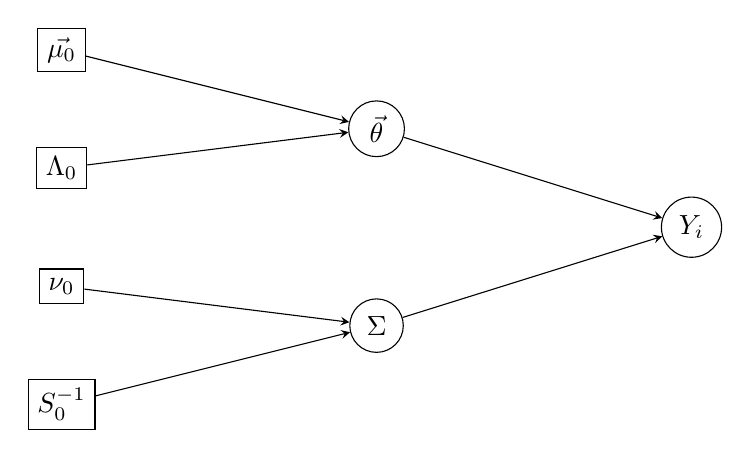
\begin{tikzpicture}[>=stealth, node distance=2cm and 4cm]
    
        % Define nodes in the first column (left)
        \node[draw, rectangle] (A1) at (0,0) {$\vec{\mu_0}$};
        \node[draw, rectangle] (A2) at (0,-1.5) {$\Lambda_0$};
        \node[draw, rectangle] (A3) at (0,-3) { $\nu_0$ };
        \node[draw, rectangle] (A4) at (0,-4.5) { $ S_0^{-1} $ };
        
        % Define nodes in the second column (middle)
        \node[draw, circle] (B1) at (4,-1) {$\vec{\theta}$};
        \node[draw, circle] (B2) at (4,-3.5) {$\Sigma$};
        
        % Define node in the third column (right)
        \node[draw, circle] (C1) at (8,-2.25) {$Y_{i}$};
        
        % Draw arrows connecting the first column to the second column
        \draw[->] (A1) -- (B1);
        \draw[->] (A2) -- (B1);
        \draw[->] (A3) -- (B2);
        \draw[->] (A4) -- (B2);
        
        % Draw arrows connecting the second column to the third column
        \draw[->] (B1) -- (C1);
        \draw[->] (B2) -- (C1);
    
    \end{tikzpicture}
\end{center}